\section{Experiments}\label{sec:experiments}
% summary

% benchmark algorithm
To benchmark the performance of MLEMTRL, we compare ourselves to a posterior sampling method (PSRL)~\citep{osband2013more}, equipped with a combination of product-Dirichlet and product-NormalInverseGamma priors for the tabular setting, and Bayesian Multivariate Regression prior~\citep{minka2000bayesian} for the continuous setting. In PSRL, at every round, a new model is sampled from the prior, and it learns in the target MDP from scratch. Finally, for model-based planning we use \textsc{RiccatiIterations}~\citep{willems1971least} to obtain the optimal linear controller for the sampled model. The experiments are deployed in \textsc{Python 3.7}, with support of \textsc{SciPy}~\citep{virtanen2020scipy}, and ran on a i5-4690k CPU and a GTX-960 GPU. 

The objectives of our empirical study are two-fold:
\begin{enumerate}
    \item How does \textsc{MLEMTRL} using impact performance in terms of \textbf{learning speed}, \textbf{jumpstart improvement} and \textbf{asymptotic convergence} compared to our baseline?
    \item What is the performance loss of \textsc{MLEMTRL} with increasing \textbf{model dissimilarity} between the estimated model and the target model?
\end{enumerate}

We conduct two kinds of experiments to verify our hypotheses. Firstly, in Figure~\ref{fig:time}, we compare the performance of MLEMTRL to PSRL~\citep{osband2013more} in terms of learning speed and jumpstart improvement. We also identify a zero or near-zero regret for MDPs satisfying the realisability conditions in Section~\ref{subsec:realisable}. Lastly, we see a trend of increase in regret with an increase in \emph{Kullback-Leibler divergence} of the true MDP $\mdp^{*}$ from our estimate, $\hat{\mdp}$. In another experiment, in Figure~\ref{fig:norms}, we further verify the relation between increase in divergence and increase in regret. We begin by recalling the goals of the transfer learning problem~\citep{langley2006transfer}.

\paragraph{Learning Speed Improvement:}
A learning speed improvement would be indicated by the algorithm reaching its asymptotic convergence with less data.
 \paragraph{Asymptotic Improvement:}
 An asymptotic improvement would mean the algorithm converges asymptotically to a superior solution to that one of the baseline.
\paragraph{Jumpstart Improvement:}
A jumpstart improvement can be verified by the behaviour of the algorithm during the early learning process. In particular, if the algorithm starts at a better solution than the baseline, or has a simpler optimisation surface, it may more rapidly approach better solutions with much less data.
\begin{figure}[t!]
    \centering
    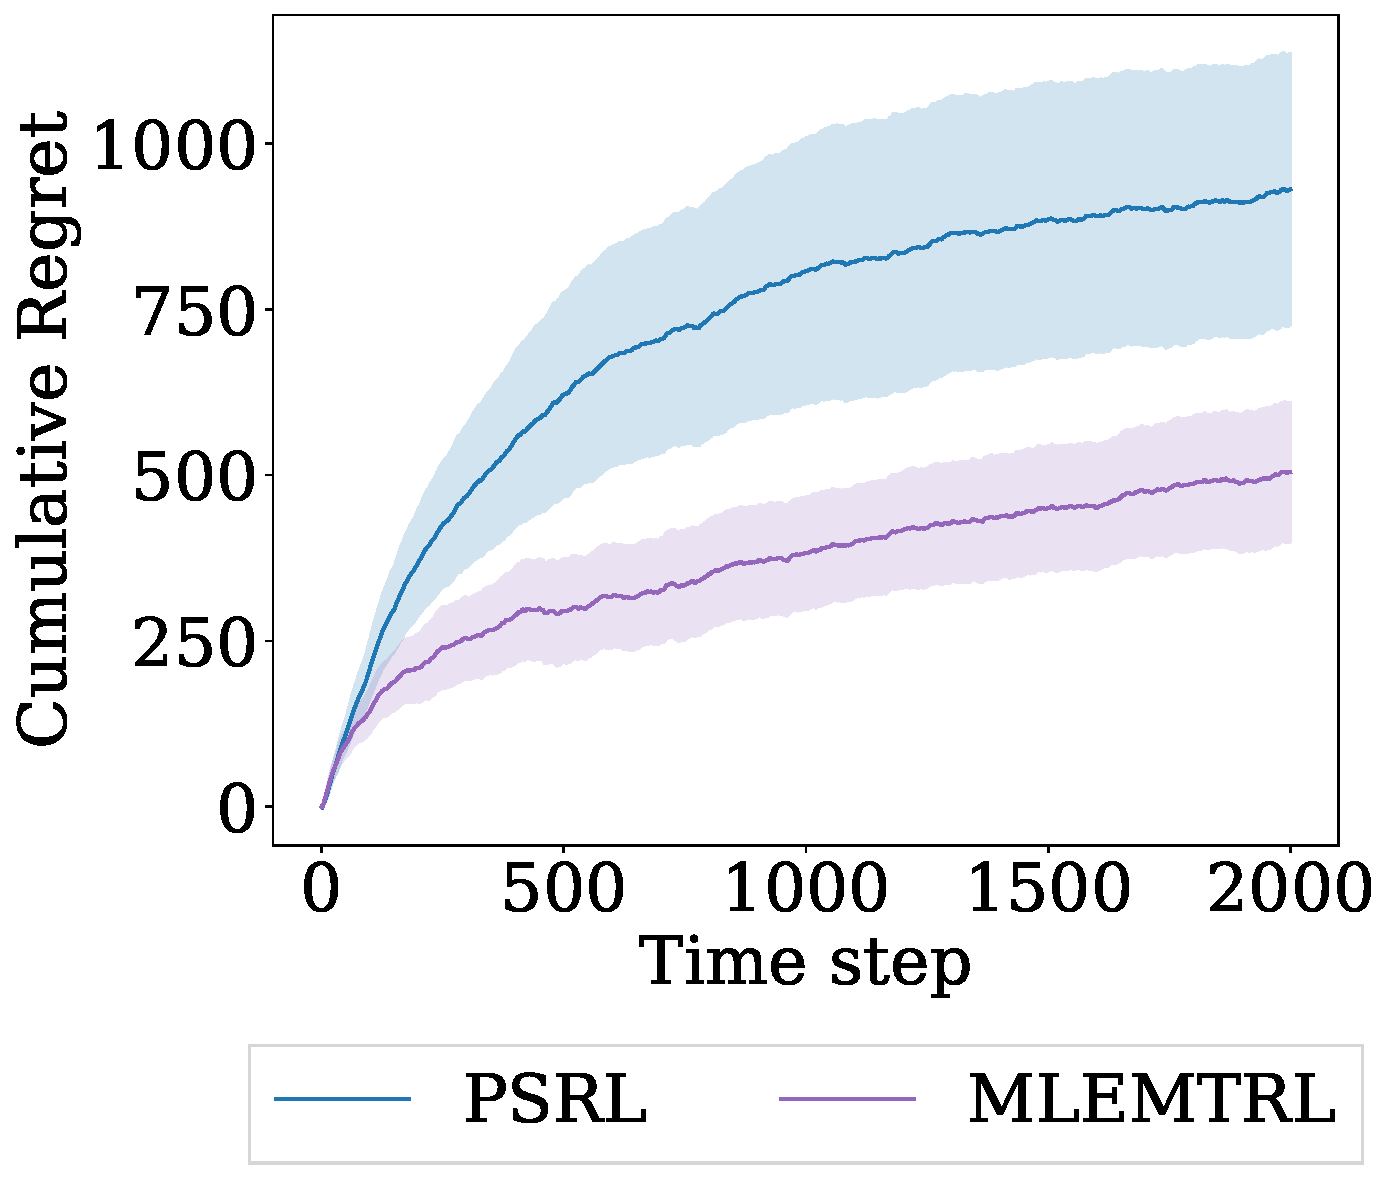
\includegraphics[width=0.4\textwidth]{img/chain_experiment.pdf}
    \caption{This visualisation is of multiple variants of the Chain environment. Here, the slippage parameter is being varied. The cumulative regret is shown over the first $2000$ time steps and the shaded regions represent the $95\%$ confidence interval of the cumulative regret for the two algorithms. The agents update their policies every $20$ steps. For regret, lower values are better.}\label{fig:chain}\vspace*{-1em}
\end{figure}
\subsection{RL Environments}
\noindent\textbf{Chain.} A common testbed for RL algorithms in tabular settings is the Chain~\citep{dearden1998bayesian} environment. In it, there is a chain of states where the agent can either walk forward or backward. At the end of the chain, there is a state yielding the highest rewards. At every step, there is a chance of the effect of the opposite action occurring. This is denoted as the \emph{slipping probability}. The slippage parameter is also what is used to create the source models, in this case, those parameters are $\{0.01, 0.20, 0.50\}$. For both algorithms, we use a product-NormalGamma prior over the reward functions. For PSRL, we use product-Dirichlet priors over the transition matrix.

\begin{figure*}[t!]
    \centering
    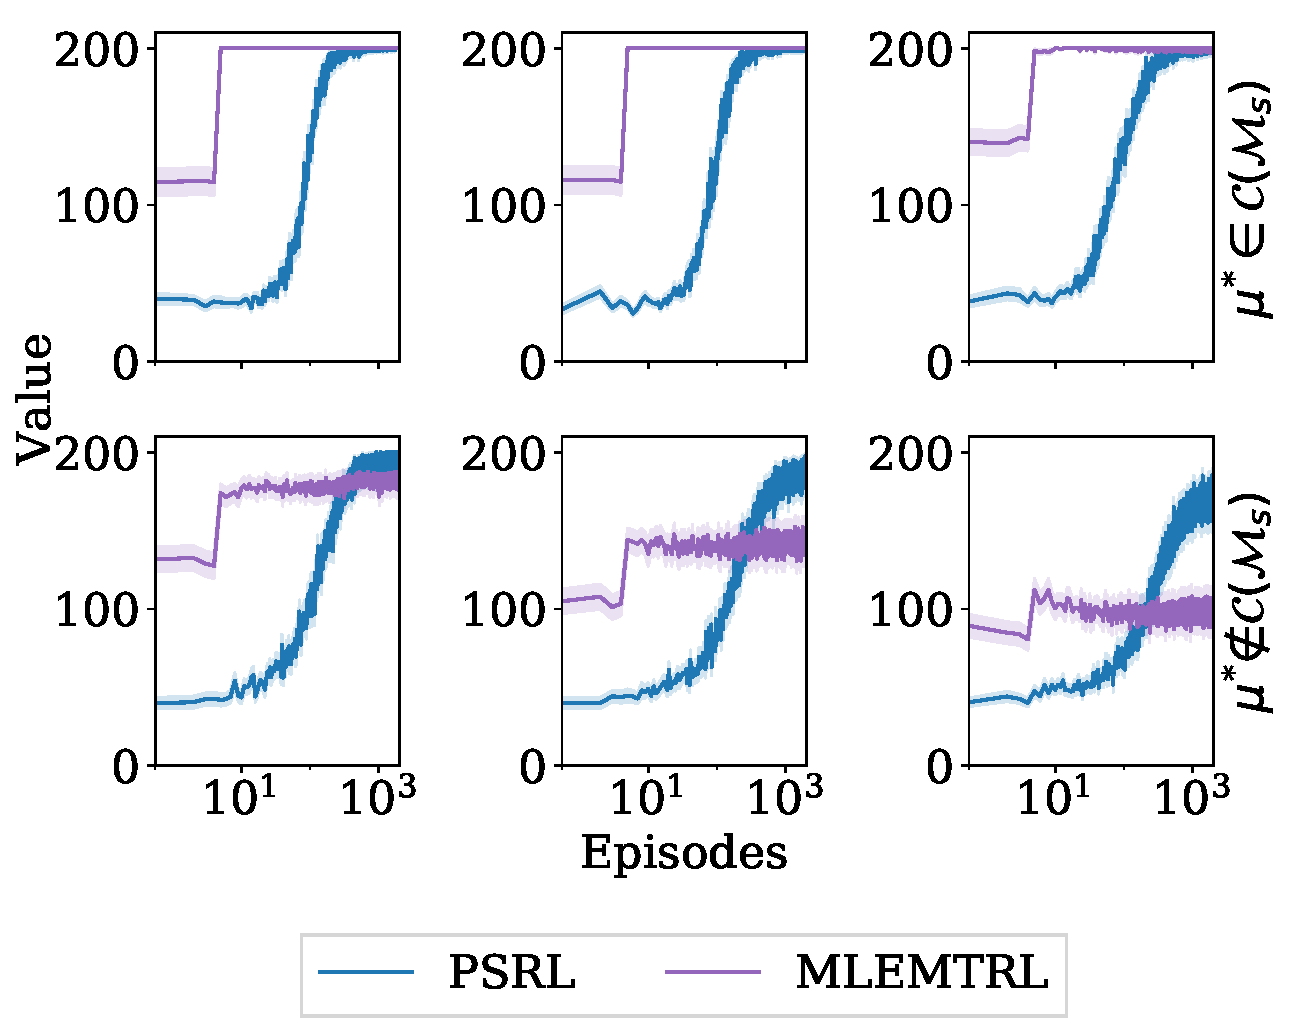
\includegraphics[width=0.5\textwidth]{img/time_experiment.pdf}
    \caption{We compare MLEMTRL against PSRL in terms of convergence speed and early performance. The value functions of the algorithms are plotted against the log of the number of episodes. The shaded area is the $68\%$ confidence of the mean over multiple MDPs with the same model dissimilarity. In the topmost row, all of the true MDPs are within the convex hull $\mathcal{C}(\mathcal{M}_s)$. In the bottom row, the MDPs are outside. As you go from top-left to bottom-right, the divergence from the true model to the average model in the convex hull increases. For utility, higher values are better.}
    \label{fig:time}
\end{figure*}


\noindent\textbf{CartPole.}
The environment used to testbed our algorithm is the \emph{Cartpole} environment~\citep{barto1983neuronlike}. The task is to stabilise a pole attached to a cart and keep it upright for the total episode length of $200$ time steps. The state-space $s \in \mathbb{R}^4$ and the action-space $a \in [-1, 1]$. A continuous action applies a bounded force in the opposite direction on the cart. The original environment parameters are the \emph{gravity} $g=9.8$, \emph{mass of cart} $m=1.0$, \emph{mass of pole} $p=0.1$ and \emph{length of pole} $l = 0.5$. In order to construct our source tasks, we create a variation of these parameters in the following way,
\[
  \mathcal{M}_s = \kbordermatrix{
    & g & m & p & l \\
    \mdp_1 & 9.80 & 1.00 & 0.10 & 0.50 \\
    \mdp_2 & 43.84 & 1.89 & 0.50 & 0.93 \\
    \mdp_3 & 46.29 & 0.34 & 0.44 & 0.13 \\
    \mdp_4 & 46.34 & 1.93 & 0.49 & 2.47 \\
    \mdp_5 & 18.95 & 2.36 & 0.37 & 1.64
  }.
\]

These source tasks are then used to transfer knowledge from to the novel task. The maximum attainable return in this environment is $200$ which happens if the agent is able to balance the pole for the full episode length. In this setting, the MLEMTRL algorithm effectively creates a mixture of linear-Gaussians as the full likelihood model and obtains the mixture weights by using experience from the novel task.
% outline

\subsection{Impacts of Model Transfer with MLEMTRL}\label{sec:impacts}
\textit{Asymptotic and Learning-speed Improvements in Tabular MDPs.} We begin by evaluating the proposed algorithm in the Chain environment. The results of said experiment is available in Figure~\ref{fig:chain}. In it, we evaluate the performance of MLEMTRL against PSRL for the first $2000$ time steps. The experiments are done by varying the slippage parameter $p \in [0.01, 0.50]$ and the results are computed for each different setup of Chain from scratch. The cumulative regret is taken w.r.t the optimal policy and the shaded regions represent the $95\%$ confidence of the cumulative regret at the time step. The confidence interval is taken over the various variations of the Chain environment. The image clearly shows MLEMTRL has a jumpstart improvement coming as a result of the transfer learning scheme but also an indication of a learning speed improvement. 

\textit{Learning-speed and Jumpstart Improvements in LQRs.} In the experiment depicted in Figure~\ref{fig:time}, we investigate the convergence rate and the jumpstart improvement of the MLEMTRL algorithm on $100$ independent target MDP realisations at six different levels of divergence. The divergence is measured from the centroid of the convex hull to the target MDP. Further, in the topmost row, all of the target MDPs belong to the convex hull of source models. As we can see, in this setting, identification of the true model occurs rapidly. One reason for this is because of the near-determinism of the environment. Compared to the agent learning from scratch, we observe zero-regret with faster convergence. As we go from top-left to bottom-right, the divergence increases. For the bottom-most row, we can again observe a faster learning rate. In this case, the degradation in performance increases with the divergence, resulting in poor performance in the final case. The experiment demonstrates that under the TRL framework, we require that the source models are not too dissimilar from the target model.


\subsection{Impact of Realisability Gap on Regret}
In the final experiment, we further illustrate the observed relation between model dissimilarity and degradation in performance. Figure~\ref{fig:norms} depicts the regret against the KL-divergence of the target model to the best proxy model in the convex set. As we can see, there is a clear connection between model dissimilarity and the performance gap in the proposed algorithm. 
This is also justified in the Section~\ref{sec:bounds} where the bounds have an explicit dependency on the model difference. Note that in the figure, only the non-zero regret experiments are shown. This is to have an idea of which models result in poor performance. As its shown, it is those models that are very dissimilar.\\~\\
\noindent\textbf{Summary of Results.} In the experiments, we sought to identify whether the proposed algorithm shows superiority in terms of the transfer learning goals given by~\citet{langley2006transfer}. In our first experiment, we see a clear superiority in terms of learning speed and jumpstart improvement. These results are consistent for the second experiment as well, given that the true MDP is similar enough to the source tasks. In the second and third experiment we verify the claim that a loss in performance (in terms of regret) has a strong dependence on the dissimilarity of the estimated MDP and the true MDP.

\iffalse
\begin{table*}[t]
    \centering
    \caption{}
    \begin{tabular}{c c c c c c }
        Type & & & $0^{+} \leftarrow  D_{\textrm{KL}}(\mdp^{*} \, || \, \mdp) \rightarrow \infty$&  & \\ \hline
          $\mdp_t \in \Delta$ & $0.00\pm 0.00$& $0.01\pm 0.01$& $0.09\pm 0.05$& $0.11\pm 0.06$& $0.11\pm 0.07$ \\
          $\# \textrm{ MDPs}$& $\#26$ & $\#370$& $\#777$& $\#824$& $\#679$ \\ \\
          $\mdp_t \notin \Delta$ & $32.83\pm 1.57$& $42.58\pm 2.14$& $75.75\pm 9.15$& $123.57\pm 11.90$& $138.49\pm 14.15$\\
           $\# \textrm{ MDPs}$& $\#2332$& $\#1283$& $\#241$&$\#159$&$\#97$\\
    \end{tabular}
\end{table*}
\fi



\begin{figure}[t!]
    \centering
    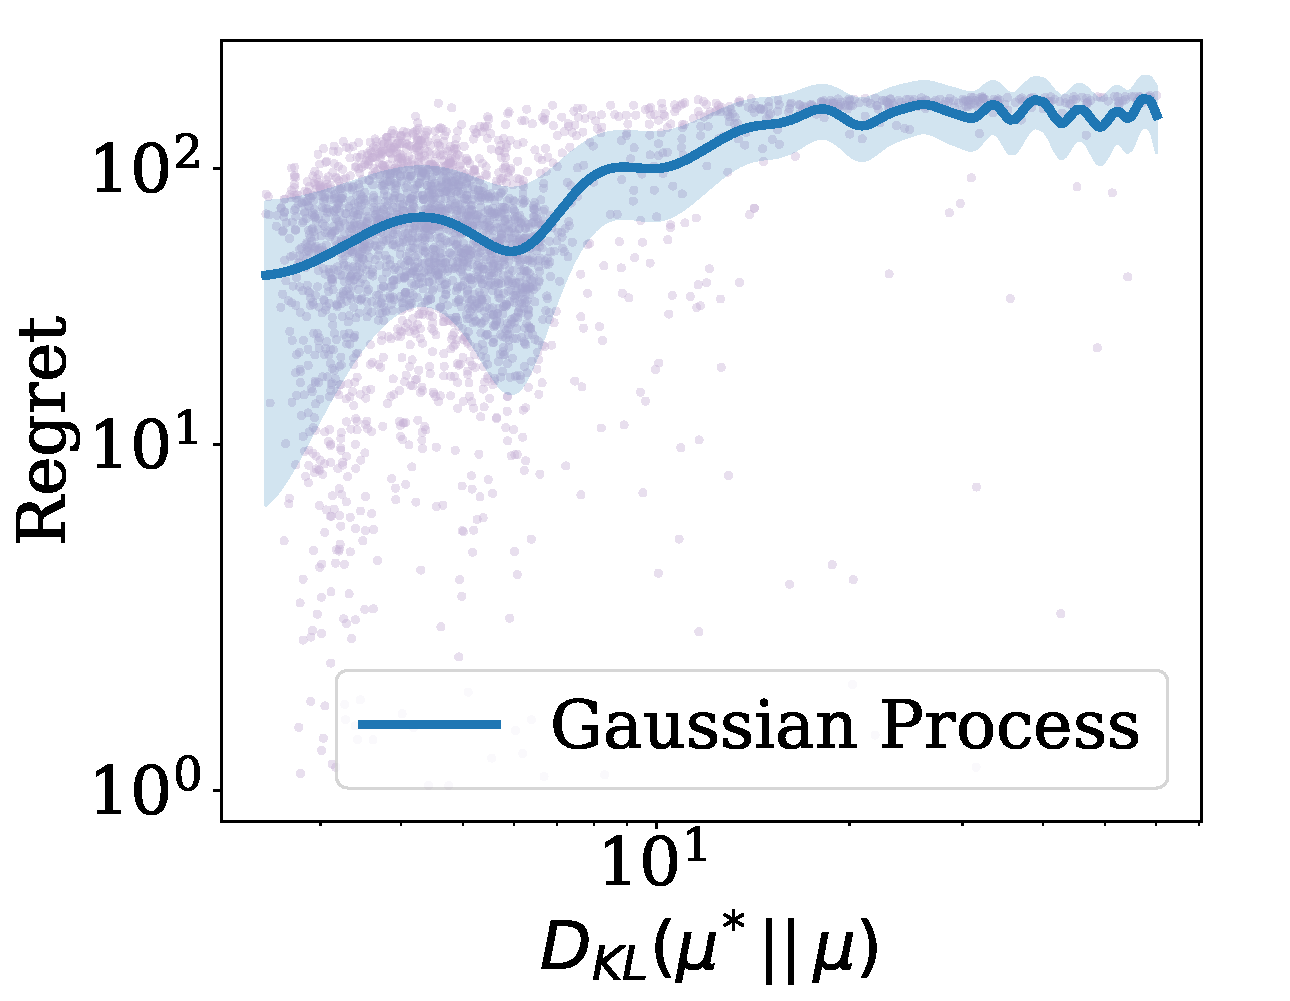
\includegraphics[width=0.4\textwidth]{img/alpha_norms}
    \caption{A log-log plot depicting the regret against the KL-divergence between the true MDP and the best proxy model. Only the non-zero regret results are displayed to indicate how sub-optimal performance relates to model dissimilarity. The thick blue line is a Gaussian Process regression model fitted on the observed data (in purple). The shaded area is the $68\%$ confidence interval of the mean.}
    \label{fig:norms}
\end{figure}